\chapter{Attenuation}
\label{ch:atten}
\newcommand{\Rhyp}{R_{\mathrm{hyp}}}
\newcommand{\Repi}{R_{\mathrm{epi}}}
\newcommand{\Rrup}{R_{\mathrm{rup}}}
\newcommand{\Rjb}{R_{\mathrm{jb}}}

\section{Overview}

Attenuation models give a measure of the level of motion observed
at some distance $R$ from an event of magnitude $r_m$. Typically
the motion of interest is a displacement, velocity or
acceleration. It is common to consider both the motion at the
ground surface as well as the motion experienced by a range of
buildings, typically approximated by single-degree of freedom
oscillators (SDOF). Such measures of motion are known as response
spectral displacement\index{response spectral displacement}, the
response spectral velocity\index{response spectral velocity} and
the response spectral acceleration\index{response spectral
acceleration} for displacement, velocity and acceleration
respectively. The most frequently used measure of motion in the
EQRM application is the response spectral
acceleration\index{response spectral acceleration} which is
described in more detail in \aref{app:RSA}. The response spectral
acceleration is denoted by $S_a(T_o,r_m,R)$ where the $T_o$ refers
to fundamental period (\aref{app:RSA}), $r_m$ refers to earthquake
magnitude (\sref{sec:magnitude_selection}) and R represents the
distance between the event and site of interest and can be any one
of $\Rhyp$, $\Repi$, $\Rrup$ or $\Rjb$ (\sref{sec:attn-dist}).

\subsection{Background theory}
\label{sec:attn-dist}


Different measures of distance are used by different attenuation
formulae. They are illustrated in \Fref{fig:attn-distances} and
can be summarised as follows (see \citet*{dr_Abrahamson97a} for
further information):

\begin{itemize}
\item {\bfseries Hypocentral} distance $\Rhyp$: from site to the hypocentre of
  the fault rupture.
\item {\bfseries Epicentral} distance $\Repi$: from site to the
vertical projection of
  the hypocentre to the ground surface (the epicentre).
\item {\bfseries Rupture distance} distance $\Rrup$: from site to closest
  point on rupture plane.
\item {\bfseries Joyner-Boore} distance $\Rjb$: from site to
closest point of the vertical projection of the rupture plane.
\end{itemize}

\begin{figure}[htp]
 \centering \psfrag{Rjb}{$\Rjb$}
\psfrag{Rhyp}{$\Rhyp$} \psfrag{Rrup}{$\Rrup$}
\psfrag{Repi}{$\Repi$} \psfrag{site}{site} \psfrag{fault}{fault}
\psfrag{d}{$h$}
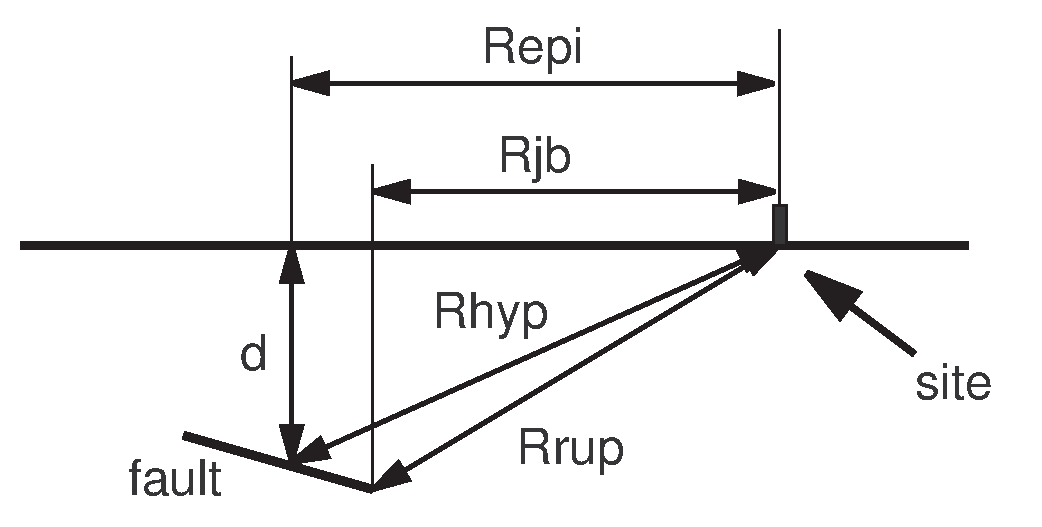
\includegraphics[width=0.7\textwidth]{diags/fig-hattn-distance}
\caption{Diagram showing the distance measures used in various
  attenuation formulae.}
  \label{fig:attn-distances}
\end{figure}

The earthquake catalogue (see \sref{ch:source}) simulates events
with moment magnitude $r_m$. However, some of the attenuation
formulas require the use of local magnitude $r_{m_l}$ (e.g.
\citealt{dr_Gaull90a}). To overcome this obstacle the following
conversion is used by \typefunc{m}{w2}{ml}
\begin{equation}
r_{m_l} =
\frac{0.473+\sqrt{0.473^2-4\times0.145(3.45-r_m)}}{2\times0.145};
\end{equation}
(Johnston, \textit{pers. comm.}, 2001) which is based on earlier
work published by the same author \citep{dr_Johnstone96a}.

\citet{dr_Boore83a} states that the uncertainties in ground motion
predictions (or estimates of the response spectral
acceleration\index{response spectral acceleration}
$S_a(T_o,r_m,R)$) can be as large as a factor of 2. He goes on to
suggest that such uncertainty can be due to variations in source
properties, propagation path and local site response. Such
uncertainty is commonly segregated into epistemic and aleatory
uncertainties (e.g \citealt{dr_Toro97a}). In this case, epistemic
uncertainty refers to that uncertainty which results from an
incomplete knowledge and data about the physics of the earthquake
process, while aleatory uncertainty is the uncertainty which
arises from the random nature of the earthquake process. Many
authors have assumed that the PDF of $S_a(T_o,r_m,R)$ for any
$(T_o,r_m,R)$ is log-normal (\citealp{dr_Campbell03a}). The EQRM
assumes that the standard deviation of the PDF is given by the
aleatory uncertainty when both aleatory and epistemic uncertainty
are provided by the attenuation model. If an attenuation model
provides only one measure of uncertainty it is assumed to be the
standard deviation. The aleatory uncertainty is then incorporated
by sampling the PDF (see \sref{attn:uncert-pdfchoice}), whereas
epistemic uncertainty is included by considering more than one
different attenuation model (see
\sref{sec:attn-multi-attnmodels}).


\subsection{Implementation}
\label{attn:implementation}

The EQRM application conducts a loop over all of the sites. Some
preparatory work is conducted before this loop 9see belwo for more
details). Inside the loop, the EQRM computes the GMPE for one site
at a time for all events and all fundamental (or RSA) periods. That
is, for each site there exists a large matrix of modelled
$S_a(T_o,r_m,R)$ whose rows correspond to the events (i.e. an
$r_m$-$R$ pair) and whose columns correspond to the $T_o$. That is

\begin{math}
%\label{fig:attn-sa-matrix}
 SA = \left[ \begin{array}{ccccc}
S_a(T_{o,1},r_{m,1},R_1) & S_a(T_{o,2},r_{m,1},R_1) &  \hdots & S_a(T_{o,N_T},r_{m,1},R_1) \\
S_a(T_{o,1},r_{m,2},R_2) & S_a(T_{o,2},r_{m,2},R_2) &  \hdots & S_a(T_{o,N_T},r_{m,2},R_2) \\
\vdots & \vdots &  \ddots & \vdots \\
S_a(T_{o,1},r_{m,N_s},R_{N_s}) & S_a(T_{o,2},r_{m,N_s},R_{N_s}) & \hdots & S_a(T_{o,N_T},r_{m,N_s},R_{N_s}) \\
\end{array} \right]
\end{math}

where $N_s$ refers to the number of events and $N_T$ refers to the
number of periods. Note that the $r_m$-$R$ pair comes from the event
catalogue (see \sref{sec:event-catalogue}) and a calculation of
distance (see \sref{sec:attn-dist}). The $T_o$ are determined by the
user-defined vector parameter \typepar{atten}{\_peri}{ods} in the
EQRM controlfile. Computationally the above calculation of GMPE is
conducted in two parts as follows:
\begin{enumerate}
\item The preparation of the attenuation coefficients
conducted before entering a loop over sites. This preparation
involves interpolating the attenuation coefficients to the
fundamental periods defined by \typepar{atten}{\_peri}{ods}. \item
The computation of the $S_a(T_o,r_m,R)$ at each site conducted
site-by-site within a loop over sites.
\end{enumerate}


Each GMPE returns an estimate of:
\begin{enumerate}
\item the mean of $log(S_a(T_o,r_m,R))$ (equivalent to the
logarithm of the median of $S_a(T_o,r_m,R)$) and hereafter denoted
by $\mu_{log(S_a)}(T_o,r_m,R)$ or $\mu_{log(S_a)}$ for brevity,
and \item the standard deviation of $log(S_a(T_o,r_m,R))$,
hereafter denoted by \newline $\sigma_{log(S_a)}(T_o,r_m,R)$ or
$\sigma_{log(S_a)}$ for brevity.
\end{enumerate}
Note that the $\sigma_{log(S_a)}$ returned by the different GMPEs
differ in the sense that they consider the variability resulting
from a range of different `causes'. A brief discussion of these
subtleties is left to the relevant section of each GMPE (see below).
A more detailed explanation of the subtleties can be found in the
relevant literature.

The distance between a site and all the events in the earthquake
catalogue is computed by ........... Recall that in the description
of an event (see \tref{tab:evntdb-columns}) there was no mention of
an event hypocentre or epicentre. Note that the hypocentre of an
actual event is defined as the point at which a rupture initiates
\citep{dr_Kramer96a} and is hence rarely located in the centre of
the rupture plane (as illustrated in Figure 2 by
\citet{dr_Sibson03a}). There are two obvious techniques that could
be used to approximate $\Repi$ and $\Rhyp$. The first technique
approximates $\Repi$ and $\Rhyp$ using $\Rjb$ and $\Rrup$
respectively. This technique is conservative since \mbox{$\Repi \geq
\Rjb$} and \mbox{$\Rhyp \geq \Rrup$}. The second technique involves
approximating $\Rhyp$ by using the distance to the rupture centroid
and $\Repi$ with the distance to the vertical surface projection of
the rupture centroid. The EQRM application currently uses the first
(i.e. conservative) technique. However, it should be noted that this
introduces a bias in the results, particularly since the GMPEs
themselves are most likely determined from events that have been
located as point sources. It is recommended that the technique for
such distance approximation is re-considered in the future. In
particular, \citet{dr_Bommer05a} provide a good discussion of
problems associated with using multiple GMPE formulae in PSHA and
\citet{dr_Scherbaum04a} provide distance metric conversion formulae
that may be used to overcome the bias issues discussed above.


\section{Ground Motion Prediction Equations}
\label{attn:atten-formula}


There are many GMPE described in the literature. A subset of these
are available for use within the EQRM application. Analogous to the
use of source models, the EQRM allows the user to use one or more
attenuation models. This section discusses the individual
attenuation formulae. The sampling of GMPE probability density
function (aleatory uncertainty) is discussed in
\sref{attn:uncertainty} and the use of multiple GMPEs is described
in \sref{sec:attn-multi-attnmodels}.


\subsection{Toro97 GMPE}

The \citet{dr_Toro97a} GMPE used in the EQRM code is based on the
Joyner-Boore distance $\Rjb$ and moment-magnitude. Note that this
reference largely describes the variability and not how the
coefficients were derived. \citet{dr_EPRI93a} describes how the
coefficients were derived.

The \citet{dr_Toro97a} GMPE divides North America into two regions
(Gulf and Mid-Continent) and can  be used with two different
measures of magnitude (local and moment). Currently the EQRM can
only use the Mid-Continent -- moment magnitude version of the
attenuation model. This version of the attenuation model is used
because the earthquake mechanism in Mid-Continent USA is believed to
be similar to that in Australia (i.e. both are intraplate settings).


The attenuation formula is
\begin{equation}
\begin{split}
\mu_{log(S_a)}(T_o,r_m,\Rjb) &= C_1 + C_2(r_m-6) + C_3(r_m-6)^2 - C_4\ln(R_M) \\
       &\quad  - (C_5-C_4)\max\left[\ln\left(\frac{R_M}{100}\right),0\right] -C_6R_M,
\end{split}
\end{equation}
where
\begin{equation}
 R_M = \sqrt{ \Rjb + C_7^2 }.
\end{equation}

The coefficients used in the code, $C_1,\ldots,C_7$, are functions
of $T_o$ and are tabulated in \citet[Table 2]{dr_Toro97a}.

The `uncertainty parameter' ($\sigma_{log(S_a)}$) can be
decomposed as follows:
\begin{equation}
 \sigma_{log(S_a)}(T_o,r_m,\Rjb) =
 \sqrt{\sigma_a(T_o,r_m,\Rjb)+\sigma_e(r_m)}.
\end{equation}

The aleatory or random uncertainty $\sigma_a$ can be separated into
a source dependant component $\sigma_{a,r_m}$ (see \citet[Table
3]{dr_Toro97a} and a path dependant component $\sigma_{a,\Rjb}$ (see
\citet[Table 4]{dr_Toro97a} as follows:
\begin{equation}
\label{eq:attn-toro-aleat} \sigma_a =
\sqrt{\sigma_{a,r_m}^2(T_o,r_m) + \sigma_{a,\Rjb}^2(T_o,\Rjb)}.
\end{equation}
The EQRM uses the aleatory uncertainty as defined by
\eref{eq:attn-toro-aleat}.

The epistemic or knowledge uncertainty $\sigma_e$ is dependant upon
source only, that is \mbox{$\sigma_e =\sigma_{e,r_m}$} (see
\citet[Page 48]{dr_Toro97a}. Note that $\sigma_{a,r_m}$ is a
function of $T_o$ and $r_m$; $\sigma_{a,\Rjb}$ is a function of
$T_o$ and $\Rjb$; and $\sigma_{e,r_m}$ is a function of $r_m$ only.

\subsection{Gaull90}
\label{attn:atten-formula-Gaull}

The \citet{dr_Gaull90a} GMPE, as used in the EQRM code, is based on
hypocentral distance $\Rhyp$ and local magnitude $r_{m_l}$. In the
paper it can be used to compute (i) the mean of the logarithm of PGA
$\mu_{log(PGA)}$ or (ii) the mean of the logarithm of the Modified
Mercalli Intensity $\mu_{log(\Imm)}$. Only the PGA is coded in the
EQRM at this stage. The formula is based on empirical intensity data
in the Australian region and the PGA extension created using Papua
New Guinea data. For the purpose of this GMPE the Australian region
is divided into four sub-regions, Western Australia, Southeastern
Australia, Northeastern Australia and Indonesia. Only the WA region
is available in the EQRM at this stage. The attenuation formulae is:
\begin{equation}
lnY = \ln a-c\ln \Rhyp + br_{m_l}
\end{equation}
where $a$, $b$ and $c$ are constants, $r_{m_l}$ is the local
magnitude of the rupture and $lnY$ represents $\mu_{log(PGA)}$ or
$\mu_{log(MMI)}$ depending on the value of the constants. The
constants are tabulated in \citet[Table 4]{dr_Gaull90a}.

Note that in the case of the \citet{dr_Gaull90a} attenuation model
(PGA version) there is no need to prepare the attenuation
coefficients because the attenuation model is only defined for
$T_o=0 sec$ (PGA). To compute $S_a(T_o,r_m,R)$ (more specifically,
$\mu_{log(S_a)}$), we can extend the $PGA$ estimate using the
Australian Standard Response Spectral Acceleration
\citep{dr_Standards93a}.

\citet[Table 4]{dr_Gaull90a} tabulate the `uncertainty
parameter(s)' ($\sigma_{log(Y)}$) and indicate that they do not
depend on $r_{m_l}$ or $\Rhyp$. Furthermore, when extending the
PGA estimate to a complete $S_a$ it is assumed that
$\sigma_{log(S_a)}$ is not a function of $T_o$ and that
\begin{equation}
\sigma_{log(S_a)}(T_o) = \sigma_{log(PGA)}.
\end{equation}
Personal discussions with Brian Gaull (2002 and 2003) have
revealed that the following values of $\sigma_{log(Y)}$; 0.7 (for
PGA) and 0.925 (for $\Imm$) should be used in preference to the
published values of 0.28 and 0.37 respectively.


\subsection{Atkinson97}

The \cite{dr_Atkinson97a} GMPE, as used in the EQRM code, is based
on hypocentral distance $\Rhyp$ and moment magnitude $r_m$. The
formula is
\begin{equation}
\mu_{log(S_a)}(T_o,r_m,\Rhyp) = C_1 + C_2(r_m-6) + C_3(r_m-6)^2
-ln(\Rhyp)-C_4\Rhyp.
\end{equation}
The coefficients used in the code, $C_1,\ldots,C_7$, are functions
of $T_o$ and are tabulated in \citet[Table 1]{dr_Atkinson97a}.

The uncertainty is dependant on $T_o$ only and is defined by
\citet{dr_Atkinson95b}. It represents aleatory uncertainty,
$\sigma_a$ and no attempt is made to separate it into into source
and path components (see \citealt[Table 2]{dr_Atkinson95b}).


\subsection{Sadigh97}

The \cite{dr_Sadigh97a} GMPE, as used in the EQRM code, is based on
rupture distance $\Rrup$ and moment-magnitude $r_m$. Using the
convention defined by \citet{dr_Campbell03a} (in accompanying
appendix), the GMPE is
\begin{equation}
\begin{split}
\mu_{log(S_a)}(T_o,r_m,\Rrup) & = C_1F +C_2 + C_3r_m
+C_4(8.5-r_m)^2 + \\ c_5ln(r_{rup}+C_7\exp{c_8r_m}) +
C_rln(r_{rup}+2),
\end{split}
\end{equation}
where the parameter $F$ is hard wired in the EQRM to 1 (hence
assuming reverse faulting). The coefficients used in the code,
$C_1,\ldots,C_7$, are functions of $T_o$ and $ r_m$. They are
tabulated in \citet[Table 2]{dr_Sadigh97a}.

\cite{dr_Sadigh97a} define a magnitude $r_m$ and period $T_o$
dependant `standard error' $\sigma(r_m,T_o)$ (see \citealt[Table
3]{dr_Sadigh97a}) which can be generalised as follows
\begin{equation}
\sigma(r_m,T_o) = \left \{ \begin{array}{ll}
C_{10}-C_{11}r_m & \textrm{for $0<r_m<7.21$} \\
c_{12} & \textrm{for $r_m \geq 7.21$} \\
\end{array} \right.
\end{equation}
where the coefficients $C_{10}$, $C_{11}$ and $C_{12}$ are functions
of $T_o$, and are defined in \cite[Table A-14]{dr_Campbell03a}. For
the purpose of consistency, $\sigma(r_m,T_o)$ is assumed to be the
aleatory uncertainty $\sigma_a$.


\subsection{Somerville09}
\textbf{Complete this section}
\begin{itemize}
\item decsribe the two options available (NonCratonic and Yilgarn)
\item cite the report
\item create table with the NonCratonic coeeficients (i.e.
\tref{tab:Somerville09_Non_Cratonic})
\end{itemize}

\begin{table}
\caption{Coeeficients for \texttt{Somerville09\_Non\_Cratonic}. The
Non-Cratonic model represents an everage model for all non cratonic
regions of Australia (\textbf{update citation}. For all practical
purposes it can be used in all regions except the Yilgran Craton.
The complete table of coefficients is include here because it was
omitted from the original publication where it should have been
table 7-3g.} \label{tab:Coeff-Somerville09_Non_Cratonic}
\footnotesize
\begin{tabular}{ccccccccc}
 \hline
Period  & $C_1$    & $C_2$     & $C_3$     & $C_4$     & $C_5$    & $C_6$    & $C_7$    & $C_8$ \\
\hline
PGA     & 1.03780  & -0.03970  & -0.79430  & 0.14450   & -0.00618 & -0.72540 & -0.03590 & -0.09730 \\
0.010   & 1.05360  & -0.04190  & -0.79390  & 0.14450   & -0.00619 & -0.72660 & -0.03940 & -0.09740 \\
0.020   & 1.05680  & -0.03920  & -0.79680  & 0.14550   & -0.00617 & -0.73230 & -0.03930 & -0.09600 \\
0.030   & 1.13530  & -0.04790  & -0.80920  & 0.15000   & -0.00610 & -0.76410 & -0.05710 & -0.09210 \\
0.040   & 1.30000  & -0.07020  & -0.83150  & 0.15920   & -0.00599 & -0.82850 & -0.09810 & -0.08530 \\
0.050   & 1.47680  & -0.09310  & -0.83330  & 0.15600   & -0.00606 & -0.86740 & -0.12740 & -0.09130 \\
0.075   & 1.70220  & -0.05160  & -0.80720  & 0.14560   & -0.00655 & -0.87690 & -0.10970 & -0.08690 \\
0.100   & 1.65720  & 0.15080   & -0.77590  & 0.13100   & -0.00708 & -0.77830 & 0.01690  & -0.05980 \\
0.150   & 1.94440  & -0.09620  & -0.75000  & 0.11670   & -0.00698 & -0.69490 & -0.13320 & -0.12530 \\
0.200   & 1.82720  & -0.06230  & -0.73430  & 0.11940   & -0.00677 & -0.64380 & -0.09570 & -0.11920 \\
0.250   & 1.74380  & -0.02530  & -0.72480  & 0.11950   & -0.00646 & -0.63740 & -0.06250 & -0.11650 \\
0.3003  & 1.80560  & -0.27020  & -0.73190  & 0.13490   & -0.00606 & -0.66440 & -0.17470 & -0.14340 \\
0.400   & 1.88750  & -0.37820  & -0.70580  & 0.09960   & -0.00589 & -0.58770 & -0.24420 & -0.21890 \\
0.500   & 2.03760  & -0.79590  & -0.69730  & 0.11470   & -0.00565 & -0.59990 & -0.48670 & -0.29690 \\
0.750   & 1.93060  & -0.80280  & -0.74510  & 0.11220   & -0.00503 & -0.59460 & -0.50120 & -0.34990 \\
1.000   & 1.60380  & -0.47800  & -0.86950  & 0.07320   & -0.00569 & -0.41590 & 0.06360  & -0.33730 \\
1.4993  & 0.47740  & 0.90960   & -1.02440  & 0.11060   & -0.00652 & -0.19000 & 1.09610  & -0.10660 \\
2.000   & -0.25810 & 1.37770   & -1.01000  & 0.10310   & -0.00539 & -0.27340 & 1.50330  & -0.04530 \\
3.0003  & -0.96360 & 1.14690   & -0.88530  & 0.10380   & -0.00478 & -0.40420 & 1.54130  & -0.11020 \\
4.000   & -1.46140 & 1.07950   & -0.80490  & 0.10960   & -0.00395 & -0.46040 & 1.41960  & -0.14700 \\
5.000   & -1.61160 & 0.74860   & -0.78100  & 0.09650   & -0.00307 & -0.46490 & 1.24090  & -0.22170 \\
7.5019  & -2.35310 & 0.35190   & -0.64340  & 0.09590   & -0.00138 & -0.68260 & 0.92880  & -0.31230 \\
10.000  & -3.26140 & 0.69730   & -0.62760  & 0.12920   & -0.00155 & -0.61980 & 1.01050  & -0.24550 \\
PGV     & 5.07090  & 0.52780   & -0.85740  & 0.17700   & -0.00501 & -0.61190 & 0.80660  & -0.03800 \\
\hline
\end{tabular}
\end{table}


\normalsize

\section{Incorporating aleatory uncertainty}
\label{attn:uncertainty}

Incorporating uncertainty is a critical component of any PSHA. The
inclusion of aleatory uncertainty in the EQRM for attenuation
 is facilitated by the EQRM controlfile parameter
 \typepar{atten}{\_variability}{\_method}.
 The aleatory uncertainty is based on estimations of
$\sigma_{log(S_a)}$ (see
\sreftwo{attn:atten-formula}{attn:implementation}).
\sreftwo{attn:uncert-randomchoice}{attn:uncert-pdfchoice} describe
two of the most commonly used techniques for incorporating
attenuation aleatory uncertainty when using the EQRM.
\tref{tab:attn-varmethods} illustrates all of the aleatory
uncertainty options that are available with the EQRM.
\begin{table}
\caption{Different techniques for incorporating attenuation
variability in the EQRM.} \vspace{0.8em}
\label{tab:attn-varmethods}
\begin{centering}
\begin{tabular}{c|p{0.7\textwidth}}
\typeparcaption{var}{\_attn}{\_method} & Description \\
\hline
None & No sampling \\
1 & PDF sampling or spawning (see \sref{attn:uncert-pdfchoice}) \\
2 & random sampling (see \sref{attn:uncert-randomchoice}) \\
3 & $+2\sigma$ from median\\
4 & $+\sigma$ from median\\
5 & $-\sigma$ from median\\
6 & $-2\sigma$ from median\\
\hline
\end{tabular}
\end{centering}
\end{table}




\subsection{Random sampling of a response spectral acceleration\index{response spectral acceleration}}
\label{attn:uncert-randomchoice}

This technique involves selecting a single `random' response
spectral acceleration\index{response spectral acceleration}
($S_a$) from its PDF by:
\begin{enumerate}
\item Selecting a random number $n_{rand}$ from the standard
normal distribution $ N \sim (0,1)$. \item Computing the $S_a$ as
follows
\begin{equation}
\label{attn:attn-var} log(A_{S_a}(T_o,r_m,R)) = \mu_{log(S_a)} +
n_{rand} \sigma_{log(S_a)},
\end{equation}
where $\sigma_{log(S_a)}$ is usually assumed to be $\sigma_a$.
\end{enumerate}

\begin{figure}
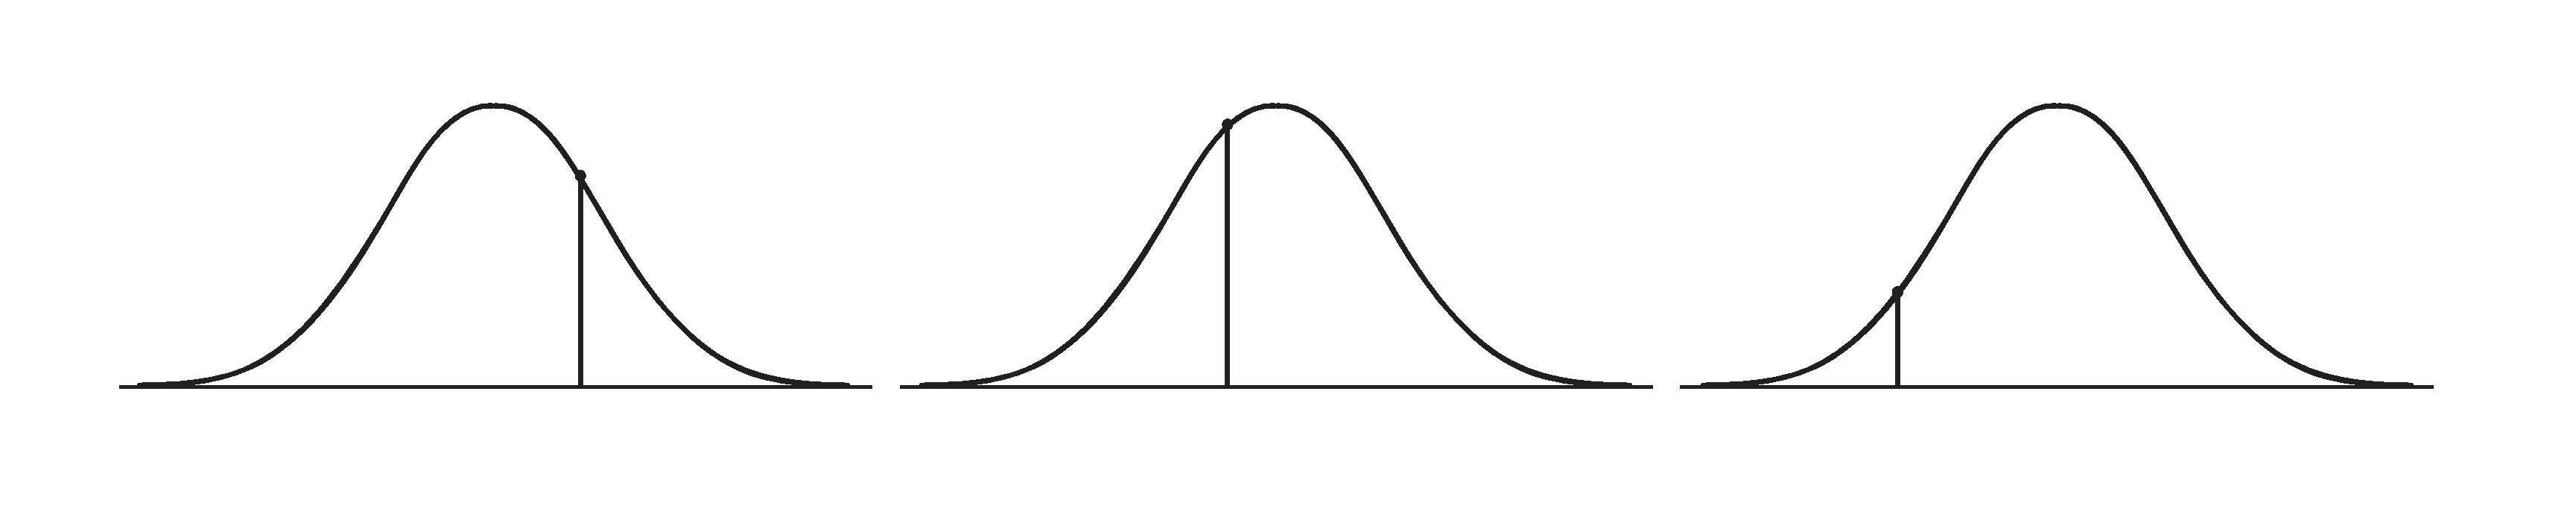
\includegraphics[width=1\textwidth]{diags/fig-hattn-random}
\caption{Selection of three different random samples from a PDF.}
\label{fig:hattn-randomsamp}
\end{figure}
Random sampling from a PDF is illustrated in
\fref{fig:hattn-randomsamp}. It is important to note the following
about random selection:
\begin{enumerate}
\item Two sites that are close to one another may give
dramatically different estimates of ground motion for the same
event. Earthquake hazard and risk values that are computed using
random sampling exhibit a low level of spatial correlation.
\item
The number $n_{rand}$ can theoretically take on any value between
$\pm \infty$. Therefore it is possible that estimates of $S_a$ using
\eref{attn:attn-var} can be unrealistically large. The EQRM
overcomes this problem by introducing a scaling factor
$PGA_{cut}=$\typepar{atten}{\_pga}{\_scaling\_cutoff} which is
applied to the RSA as follows:
\begin{equation}
 log(A_{S_a,new}(T_o,r_m,R)) = R_{scale} \times
log(A_{S_a,old}(T_o,r_m,R))
\end{equation}
where
\begin{equation}\label{rw}
R_{scale}  =
\begin{cases}
1,  PGA \leq PGA_{cut}\\
\frac{PGA_{cut}}{log(A_{S_a}(0,r_m,R))},
PGA > PGA_{cut}\\
\end{cases}
\end{equation}

%if PGA > \typepar{atten}{\_pga}{\_scaling\_cutoff}\\
%R_{scale} =
%\frac{\textrm{\typepar{atten}{\_pga}{\_scaling\_cutoff}}}{log(A_{S_a}(0,r_m,R))}
%\\
% log(A_{S_a,new}(T_o,r_m,R)) = R_{scale} \times
%log(A_{S_a,old}(T_o,r_m,R)).
%\end{equation}
\item There is no effort to account for the likelihood (or
probability) of selecting a particular $n_{rand}$ i.e. a particular
value of the $S_a$ is not weighted against its likelihood. It can be
argued that if enough earthquakes are simulated a range of different
$n_{rand}$ will be taken (high and low) and the overall hazard
and/or risk values will converge to the true ones.
\end{enumerate}


\subsection{Sampling the probability density function of
the response spectral acceleration\index{response spectral acceleration} (spawning)}
\label{attn:uncert-pdfchoice}


An alternative technique for incorporating uncertainty relies on
sampling the PDF of the $S_a$. This technique is used by Aon Re
(Mendez, \textit{pers. comm.}, 2003) and is often referred to as
spawning. An integral component of sampling the PDF is the
spawning of events with the event catalogue (see
\sref{source:spawning}). Essentially the approach involves taking
a user defined number of copies of each event. Every event copy is
then available for calculation of hazard (or risk) using a
different sample from the attenuation PDF.
\begin{enumerate}
\item Firstly the user must define a lower magnitude bound
$m_{bnd}$, a number of samples $n_{smples}$ and a PDF range
$n_\sigma$ (see \sref{source:spawning} for a complete definition).
Recall that \typefunc{fuse}{\_4}{hzd} redefines the event activity
$r_\nu$ using a weight $w_e$, derived by truncating and
re-normalising a standard normal distribution to $\pm n_\sigma$.
\item The $S_a$ is computed as follows
\begin{equation}
\label{attn:uncertainty-pdfsample}
\begin{array}{ll}
log(A_{S_a,i}(T_o,r_m,R)) = \mu_{log(S_a)} - \epsilon_i
\sigma_{log(S_a)}\ & \textrm{for $i=1 \ldots
n_{smples}$} \\
\end{array}
\end{equation}
where
\begin{equation}
\label{attn:uncertainty-def-epsilon}
\begin{array}{ll}
\epsilon_i = -n_\sigma + + (i-1)\Delta &
\textrm{for $i=1 \ldots n_{smples}$} \\
\end{array}
\end{equation}
and
\begin{equation}
\Delta = \frac{2n_\sigma}{n_{smples}-1}.
\end{equation}
Note that
\ereftwo{attn:uncertainty-pdfsample}{attn:uncertainty-def-epsilon}
ensure that the $S_a$ associated with each of the event copies are
evenly spread across the domain of the attenuation PDF
(\fref{fig:hattn-spawnsamp}). Recall from \sref{source:spawning}
that the event activities $r_\nu$ giving rise to each of the $S_a$
described in \eref{attn:uncertainty-pdfsample} are modified by
\typefunc{fuse}{\_4}{hzd} as follows:
\begin{equation}
r_{\nu,i} = r_{\nu,original} \times w_{e,i}
\end{equation}
\end{enumerate}

For example, assume that there is an event with $r_\nu=0.05$ that
gives rise to \mbox{$\mu_{log(S_a)}=[0.3g, 0.5g, 0.2g]$} at the
periods \mbox{$T_o = [0s,0.3s,1s]$} respectively. Also assume that
the estimates of $\mu_{log(S_a)}$ have the following standard
deviations \mbox{$\sigma_{log(S_a)}=\sigma_a = [0.03,0.04,0.01]$}.
Defining $m_{bnd}=0$, $n_{smples}=5$ and $n_\sigma=2.5$ gives
\begin{equation}
\Delta = \frac{2 \times 2.5}{5-1} = 1.25,
\end{equation}

and

%%%========================
% Automatically generated by *\diags\make_spawn_table.m
\begin{center} $ \begin{array}{ccccc}
i & w_{e,i} & \epsilon_i & r_\nu & log(A_{S_a,i}) \\
\hline
1 & 0.0219 & -2.5 & 0.0011 & [0.225g, 0.4g, 0.175g] \\
2 & 0.2285 & -1.25 & 0.0114 & [0.2625g, 0.45g, 0.1875g] \\
3 & 0.4991 & 0 & 0.025 & [0.3g, 0.5g, 0.2g] \\
4 & 0.2285 & 1.25 & 0.0114 & [0.3375g, 0.55g, 0.2125g] \\
5 & 0.0219 & 2.5 & 0.0011 & [0.375g, 0.6g, 0.225g] \\
\hline
\end{array}$
\end{center}
%%%========================

\begin{figure}
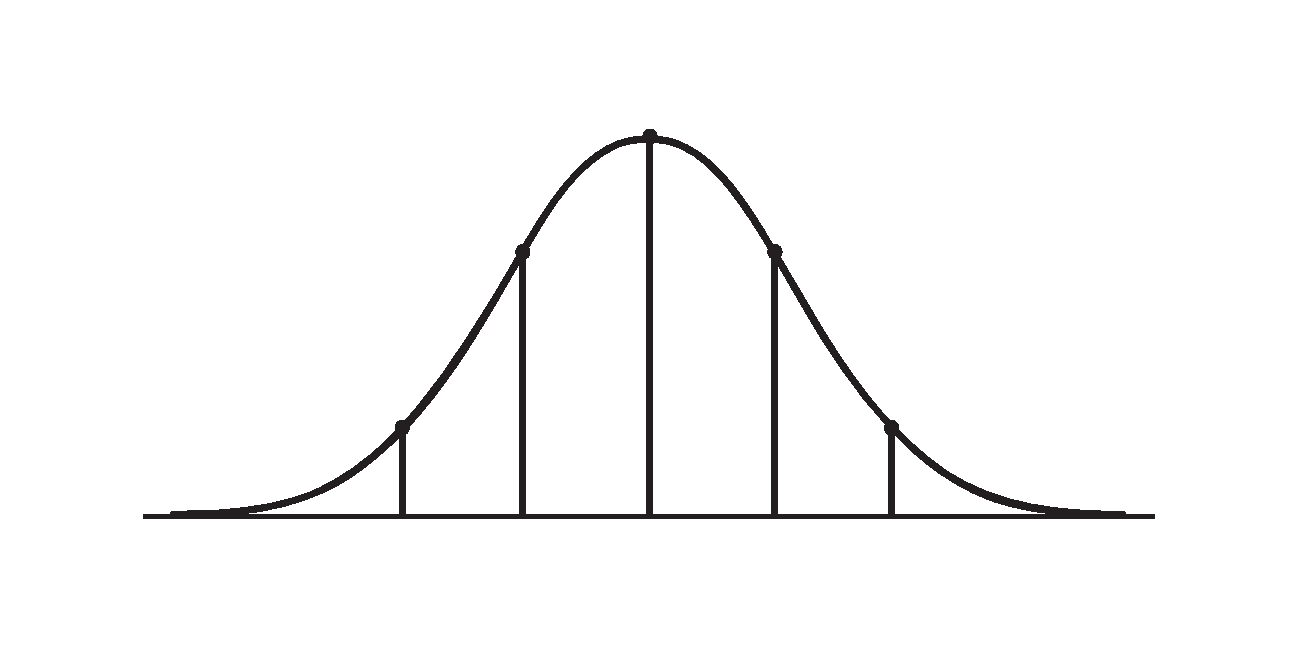
\includegraphics[width=1\textwidth]{diags/fig-hattn-spawning}
\caption{Samples drawn from a PDF using the sampling by spawning
technique with $n_{smples}=5$ and $n_\sigma=2.5$. The width
between the vertical bars is $\Delta$. Note that there is one
sample for each of the five (spawned) copies of the original
event.} \label{fig:hattn-spawnsamp}
\end{figure}

It is important to note the following about spawning:
\begin{enumerate}
\item Sub-sampling the PDF provides a smoother (and repeatable)
estimate of the $S_a$ than random selection
(\sref{attn:uncert-randomchoice}). \item The range of possible $S_a$
values is bounded by the $n_\sigma$. \item Estimates of all $S_a$
are weighted against an event activity $r_\nu$ that accounts for the
likelihood of a particular ground motion being observed. \item The
nature of spawning means that there are more evaluations of the
GMPE. This means that it is typically slower and more memory
intesive since the $S_a$ array is larger.
\end{enumerate}




\subsection{Recomendation for sampling GMPE aleatory Uncertainty}

\textbf{David to complete this section}
\begin{itemize}
\item use spawning for hazard - exaplin why
\item use random sampling for risk - exaplain why
\end{itemize}

\section{Using multiple GMPEs - Incorporating epistemic uncertainty}
\label{sec:attn-multi-attnmodels}

The use of attenuation models in the EQRM is controlled by the
\typeself{set}{da}{ta} parameter \typepar{atten}{uation}{\_flag}.
Recall from \sref{sec:application-setdata} that
\typepar{atten}{uation}{\_flag} is a two row matrix with one
column for each attenuation model to be used. The format of
\typepar{atten}{uation}{\_flag} is
\begin{center}
\begin{math}
%\label{fig:attn-sa-matrix}
 \left[ \begin{array}{ccccc}
P_1 & P_2 &  \hdots & P_n \\
w_{a,1} & w_{a,2} &  \hdots & w_{a,n} \\
\end{array} \right],
\end{math}
\end{center}
where the integers $\{P_i\}_{i=1}^n$ are pointers to the
attenuation model (see \tref{tab:attn-flags}) and the real numbers
$\{w_{a,i}\}_{i=1}^n$ are weights for the respective attenuation
models. Note that the weights $w_i$ must either be all positive or
all negative and
\begin{equation}
\left|\sum_{i=1}^{n}w_{a,i}\right| = 1.
\end{equation}



The mechanism for using more than one attenuation model is similar
to the mechanism used for spawning (see
\sref{attn:uncert-pdfchoice}). That is, the event catalogue is
copied $n$ times (once for each attenuation model) and the
appropriate attenuation model applied to its respective copy. The
values of ground motion (loss for risk) can then be treated
independently for the hazard/risk calculation (if
$\sum_{i=1}^{n}w_{a,i} = -1$) or aggregated before the hazard/risk
assessment is undertaken (if $\sum_{i=1}^{n}w_{a,i} = 1$). This
notion of logic tree collapse is described by
\fref{fig:attn-treecollapse}.


\section{Collapse versus no-collapse}

The techniques adopted for incorporating spawning (see \sref
{attn:uncert-pdfchoice}) and using multiple ground motion models are
similar in the sense that they require multiple evaluations of
ground motion for each event. These are carried through the various
stages of an EQRM simulation such as amplification, building damage
and loss calculation (see following chapters). At the end of the
simulation these values can then be collapsed back to a single `best
estimate' or kept in a un-collapsed form and used to determine the
hazard and/or risk curve (see \cref{ch:risk}). These two options are
illustrated in \fref{fig:attn-treecollapse} for both a hazrd and
risk simulation. Note that when collapsing the samples the extreme
values are removed from the hazard or risk curves. For this reason
we recomend the no-collapse option.

\begin{figure}
 \setlength{\unitlength}{1mm}
(a)  % This is the hazard tree for multi attenuation with collapse

\hspace{4em} \begin{centering}
\begin{picture}(70,30)
% middle branch
\put(0,12){$E_{ij}$} \put(7,13){\vector(1,0){15}}
\put(24,12){$Sa_{ij}^{(2)}$} \put(33,13){\vector(1,0){15}}
\put(50,12){$\widetilde{Sa_{ij}^{(2)}}$} \put(12,14){$w_2$}
% upper branch
\put(7,14){\vector(3,2){15}} \put(24,23){$Sa_{ij}^{(1)}$}
\put(33,24){\vector(1,0){15}}
\put(50,23){$\widetilde{Sa_{ij}^{(1)}}$}
\put(11,20){\rotatebox{30}{$w_1$}}
% lower branch
\put(7,12){\vector(3,-2){15}} \put(24,0){$Sa_{ij}^{(3)}$}
\put(33,1){\vector(1,0){15}} \put(50,0){$\widetilde{Sa_{ij}^{(3)}}$}
\put(11,5){\rotatebox{-30}{$w_3$}}
% concatenation at end
\put(61,5){\scalebox{1.2}[6.5]{\}}} \put(65,12){$ {\displaystyle
\widetilde{Sa_{ij}} = \sum_{k=1}^{3}w_k\widetilde{Sa_k} } $}
\end{picture}
\end{centering}

\vspace{0.8em}
(b) % This is the hazard tree for multi attenuation with NO collapse

\hspace{4em} \begin{centering}
\begin{picture}(70,30)
% middle branch
\put(0,12){$E_{ij}$} \put(7,13){\vector(1,0){15}}
\put(24,12){$Sa_{ij}^{(2)}$} \put(33,13){\vector(1,0){15}}
\put(50,12){$\widetilde{Sa_{ij}^{(2)}}$} \put(12,14){$w_2$}
% upper branch
\put(7,14){\vector(3,2){15}} \put(24,23){$Sa_{ij}^{(1)}$}
\put(33,24){\vector(1,0){15}}
\put(50,23){$\widetilde{Sa_{ij}^{(1)}}$}
\put(11,20){\rotatebox{30}{$w_1$}}
% lower branch
\put(7,12){\vector(3,-2){15}} \put(24,0){$Sa_{ij}^{(3)}$}
\put(33,1){\vector(1,0){15}} \put(50,0){$\widetilde{Sa_{ij}^{(3)}}$}
\put(11,5){\rotatebox{-30}{$w_3$}}
\end{picture}
\end{centering}

\vspace{0.8em}
(c) % This is the risk tree for multi attenuation with collapse

\hspace{4em} \begin{centering}
\begin{picture}(70,30)
% middle branch
\put(0,12){$E_{ij}$} \put(7,13){\vector(1,0){15}}
\put(24,12){$Sa_{ij}^{(2)}$} \put(33,13){\vector(1,0){15}}
\put(50,12){$\widetilde{Sa_{ij}^{(2)}}$} \put(12,14){$w_2$}
\put(60,13){\vector(1,0){15}} \put(77,12){$L_{ij}^{(2)}$}
% upper branch
\put(7,14){\vector(3,2){15}} \put(24,23){$Sa_{ij}^{(1)}$}
\put(33,24){\vector(1,0){15}}
\put(50,23){$\widetilde{Sa_{ij}^{(1)}}$}
\put(11,20){\rotatebox{30}{$w_1$}} \put(60,24){\vector(1,0){15}}
\put(77,23){$L_{ij}^{(1)}$}
% lower branch
\put(7,12){\vector(3,-2){15}} \put(24,0){$Sa_{ij}^{(3)}$}
\put(33,1){\vector(1,0){15}} \put(50,0){$\widetilde{Sa_{ij}^{(3)}}$}
\put(11,5){\rotatebox{-30}{$w_3$}} \put(60,1){\vector(1,0){15}}
\put(77,0){$L_{ij}^{(3)}$}
% concatenation at end
\put(86,5){\scalebox{1.2}[6.5]{\}}} \put(90,12){$ {\displaystyle
 L_{ij} = \sum_{k=1}^{3}w_kL_k } $}
\end{picture}
\end{centering}

\vspace{0.8em}
(d)  % This is the risk tree for multi attenuation with NO collapse


\hspace{4em}\begin{picture}(70,30)
\begin{centering}
% middle branch
\put(0,12){$E_{ij}$} \put(7,13){\vector(1,0){15}}
\put(24,12){$Sa_{ij}^{(2)}$} \put(33,13){\vector(1,0){15}}
\put(50,12){$\widetilde{Sa_{ij}^{(2)}}$} \put(12,14){$w_2$}
\put(60,13){\vector(1,0){15}} \put(77,12){$L_{ij}^{(2)}$}
% upper branch
\put(7,14){\vector(3,2){15}} \put(24,23){$Sa_{ij}^{(1)}$}
\put(33,24){\vector(1,0){15}}
\put(50,23){$\widetilde{Sa_{ij}^{(1)}}$}
\put(11,20){\rotatebox{30}{$w_1$}} \put(60,24){\vector(1,0){15}}
\put(77,23){$L_{ij}^{(1)}$}
% lower branch
\put(7,12){\vector(3,-2){15}} \put(24,0){$Sa_{ij}^{(3)}$}
\put(33,1){\vector(1,0){15}} \put(50,0){$\widetilde{Sa_{ij}^{(3)}}$}
\put(11,5){\rotatebox{-30}{$w_3$}} \put(60,1){\vector(1,0){15}}
\put(77,0){$L_{ij}^{(3)}$}
\end{centering}
\end{picture}


\caption{The application of spawning to a single synthetic
earthquake $E_{ij}$;(a) the collapse of spawned samples for hazard
(\typeparcaption{src}{\_eps}{\_switch}$=1$); (b) hazard spawning
without collapse (\typeparcaption{src}{\_eps}{\_switch}$=2$); (c)
the collapse of spawned samples for risk
(\typeparcaption{src}{\_eps}{\_switch}$=1$); and (d) risk spawning
without collapse (\typeparcaption{src}{\_eps}{\_switch}$=2$). The
illustrated procedure is repeated for $N_s$ events in the event
catalogue and the techniques of \cref{ch:risk} used to assess the
hazard or risk.} \label{fig:attn-treecollapse}
\end{figure}











%%% Local Variables:
%%% mode: latex
%%% TeX-master: "eqrmtech"
%%% End:
